\documentclass{Phyport}

\usepackage{placeins}
\usepackage{hyperref}
\usepackage{amsmath}
\hypersetup{
    colorlinks=true,
}

\exname{非平衡电桥} %实验名称
\extable{15}
\instructor{谭艾林} %指导教师
\class{github} %班级
\name{MJ} %姓名
\stuid{2025} %学号

\nyear{2025} %年
\nmonth{12} %月
\nday{29} %日
\nweekday{一} %星期几

\begin{document}
\setcounter{page}{0}
\makecover

\section{预习报告（10分）}
\subsection{实验综述（5分）}

平衡电桥一般用于测量相对稳定的物理量，要测量连续变化的电桥需要采用非平衡电桥。
实际上是相应传感器元件受到特定的外界环境变化而引起内阻变化，通过非平衡电桥将阻值转化为电压输出，
达到测量和控制环境变化的目的。

如图为非平衡电桥的结构：

\begin{figure}[htpb!]
    \centering
    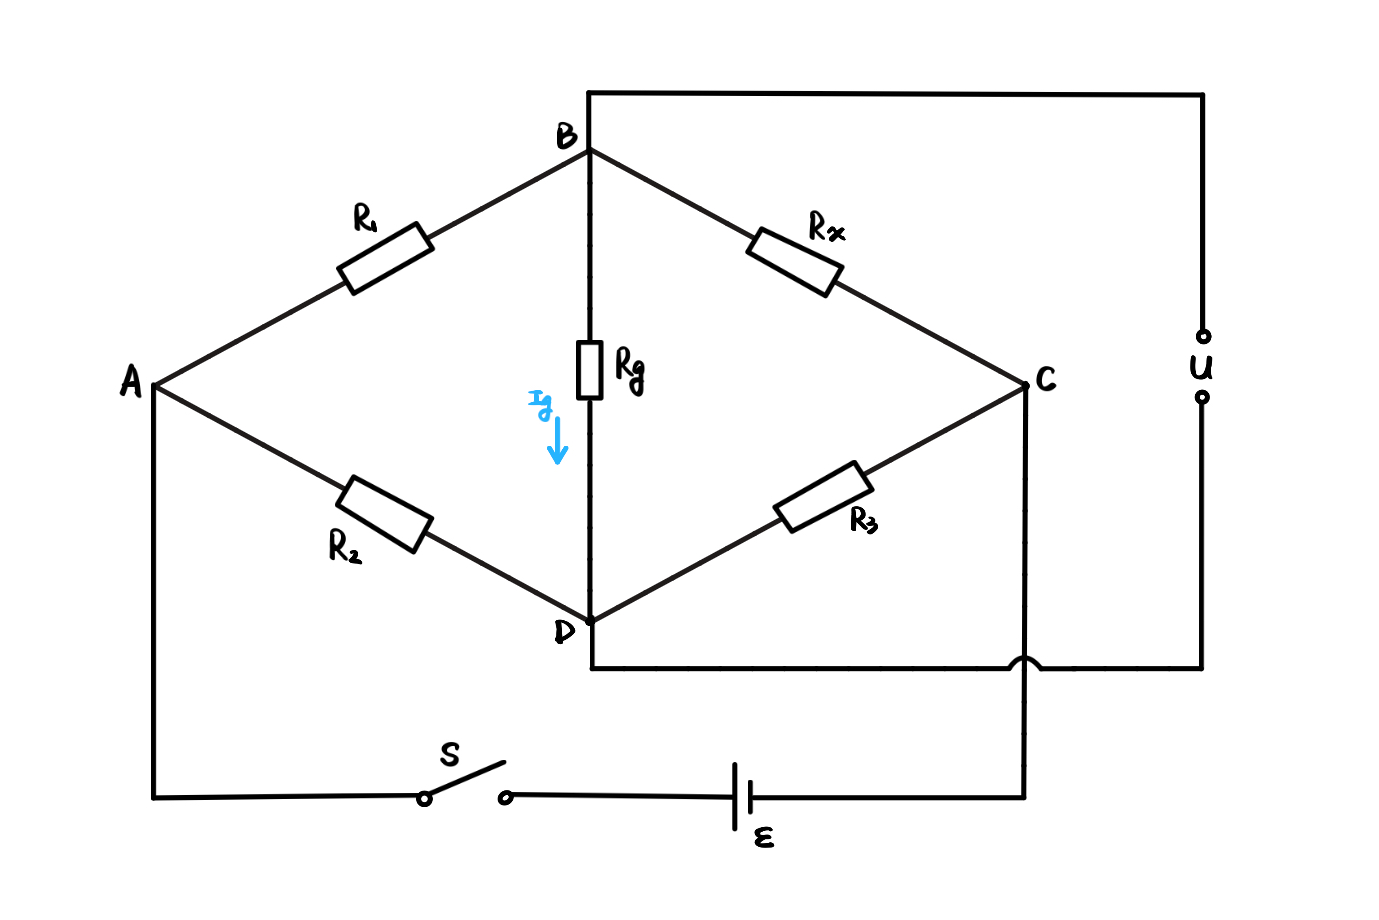
\includegraphics[width=0.35\textwidth]{demo.PNG}
\end{figure}

当负载电阻 $R_g \to \infty$ 时，有 $I_g = 0$ ，输出电压为

\[
U = U_{BC} - U_{DC} = \frac{R_2 R_x - R_1 R_3}{(R_1 + R_x)(R_2 + R_3)} \epsilon
\]

当满足 $R_1 R_3 = R_2 R_x$ 时，易知电桥输出电压为零，处于平衡状态；
而如果固定 $R_1 、 R_2 、 R_3$ ，待测电阻 $R_x$ 变为 $R_x + \Delta R_x$ 后，
电桥会因不平衡而产生输出电压：

\[
U = \frac{R_2 R_x + R_2 \Delta R_x - R_1 R_3}{(R_1 + R_x + \Delta R_x)(R_2 + R_3)} \epsilon
\]

测量这个输出电压，就可以求出电阻 $R_x$ 的变化值 $\Delta R_x$ 。

测量变温金属的电阻温度系数时，由于处于室温且温度变化不大，金属阻值随温度近似呈线性关系：

\[
R_t = R_0 (1 + \alpha t)
\]

其中 $t$ 为摄氏温度， $R_0$ 是 $t = 0 ^{\circ}C$ 的阻值， $\alpha$ 是电阻温度系数。

调节至 $R_1 = R_2 = R_3 = R_0$ 与 $R_x = R_t$ ，代入输出非平衡电压，化简后求出电阻温度系数:

\[
\alpha = \frac{4 U}{t (\epsilon - 2 U)}
\]

此外，通过平衡电桥，多次测量不同温度下平衡状态下的 $R_3$ 阻值并记录相应温度，描绘出铜电阻的温度特性曲线，
由曲线求出电阻温度系数。

\subsection{实验重点（3分）}

本实验的重点在于掌握非平衡直流电桥的工作原理和测量方法，并能够应用非平衡直流电桥测量金属材料
的温阻特性和电阻温度系数。

\subsection{实验难点（2分）}

本实验的难点主要在于要精确调节非平衡电桥的起始平衡状态，考虑电桥灵敏度；
在金属电阻温度变化的过程中控制速度，使得阻值与温度读数准确对应；以及减小接触电阻等干扰。

\section{原始数据（20分）}

实验记录数据：

\begin{figure}[htpb!]
    \centering
    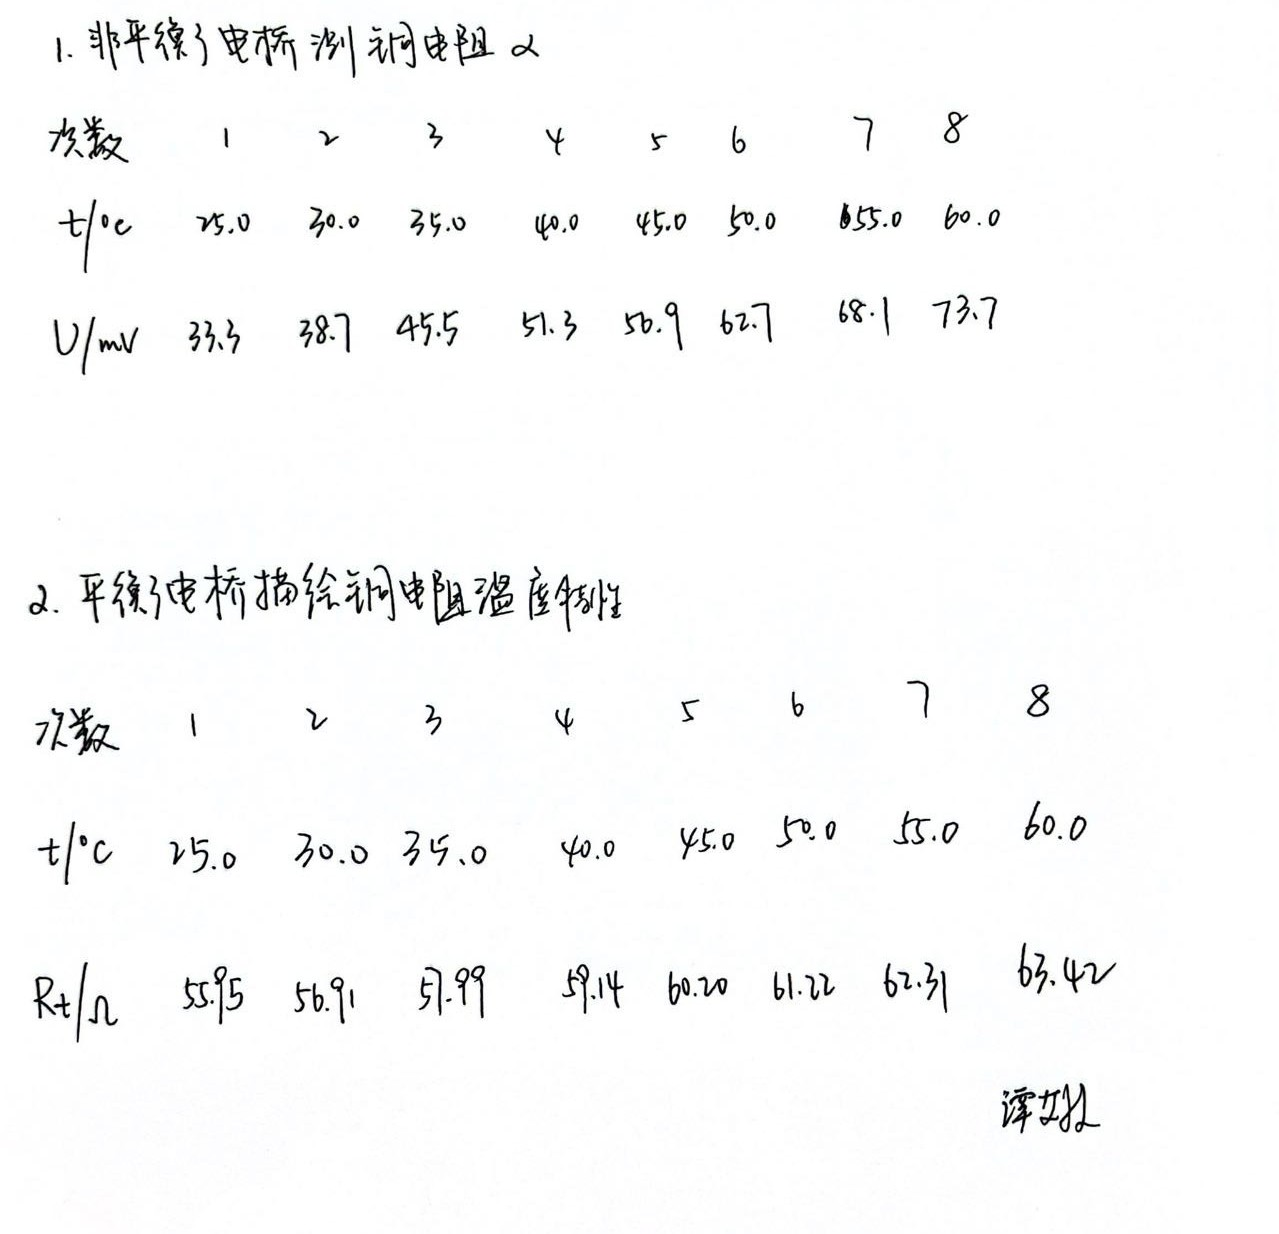
\includegraphics[width=0.9\textwidth]{data14.jpg}
\end{figure}

\FloatBarrier

\section{结果与分析（60分）}
\subsection{数据处理与结果（30分）}

\textbf{1. 用非平衡电桥测铜电阻 Cu50 温度系数}

将待测电阻 $R_x$ 和 $R_1$ 、 $R_2$ 、 $R_3$ 均设置为 $50 \Omega$ ，每间隔 $5 ^{\circ}C$ 测量非平衡电压，
记录数据如下并计算对应温度系数，其中 $\epsilon = 1.3 V$ ： 

\begin{table}[htpb!]
    \centering
    \begin{tabular}{ccccccccc}
        \hline
        实验序号 & 1 & 2 & 3 & 4 & 5 & 6 & 7 & 8 \\
        \hline
        温度 $t / ^{\circ}C$ & 25.0 & 30.0 & 35.0 & 40.0 & 45.0 & 50.0 & 55.0 & 60.0 \\
        电压 $U / mV$ & 33.3 & 38.7 & 45.5 & 51.3 & 56.9 & 62.7 & 68.1 & 73.7 \\
        $\alpha / ^{\circ}C^{-1}$ & 0.00416 & 0.00420 & 0.00433 & 0.00437 & 0.00439 & 0.00441 & 0.00441 & 0.00442 \\
        \hline
    \end{tabular}
\end{table}

计算温度系数的平均值为：

\[
\bar{\alpha} = \frac{1}{8} \sum_{i=1}^8 \alpha_i = 0.00434 ^{\circ}C^{-1}
\]

与理论值 $\alpha_0 = 0.00428 ^{\circ}C^{-1}$ 的相对误差为：

\[
E = \frac{|\bar{\alpha} - \alpha_0|}{\alpha_0} = 1.4 \%
\]

\textbf{2. 用平衡电桥描绘铜电阻 Cu50 温度特征曲线}

使用平衡电桥，每隔 $5 ^{\circ}C$ 测量不同温度下平衡状态的电阻值，数据如下：

\begin{table}[htpb!]
    \centering
    \begin{tabular}{ccccccccc}
        \hline
        实验序号 & 1 & 2 & 3 & 4 & 5 & 6 & 7 & 8 \\
        \hline
        温度 $t / ^{\circ}C$ & 25.0 & 30.0 & 35.0 & 40.0 & 45.0 & 50.0 & 55.0 & 60.0 \\
        阻值 $R_t / \Omega$ & 55.95 & 56.91 & 57.99 & 59.14 & 60.20 & 61.22 & 62.31 & 63.42 \\
        \hline
    \end{tabular}
\end{table}

用MATLAB作 $R_t - t$ 的特性曲线，得到的拟合直线为 $R_t = 0.2144 t + 50.5313 (\Omega)$ ，如图：

\begin{figure}[htpb!]
    \centering
    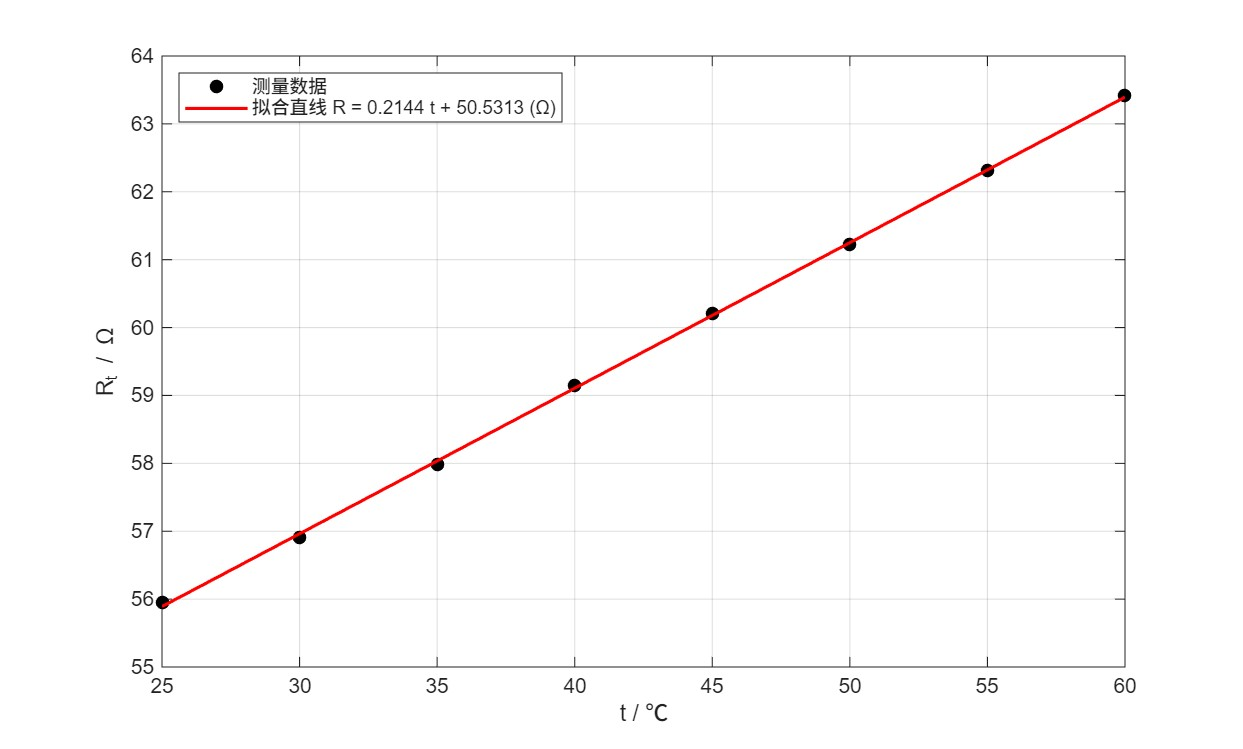
\includegraphics[width=0.65\textwidth]{fit_2result.jpg}
\end{figure}

结合公式 $R_t = R_0 (1 + \alpha t)$ 推出温度系数：

\[
\alpha = \frac{0.2144}{50.5313} = 0.00424 ^{\circ}C^{-1}
\]

与理论值 $\alpha_0 = 0.00428 ^{\circ}C^{-1}$ 的相对误差为：

\[
E = \frac{|\alpha - \alpha_0|}{\alpha_0} = 0.9 \%
\]

\subsection{误差分析（20分）}

本实验采用两种方法测量铜电阻 Cu50 的温度系数，综合来看误差都在 $1 \%$ 左右，结果较为可靠，而非平衡电桥法的误差要明显大于平衡电桥法，主要误差来源：

\begin{enumerate}
    \item 由于实验条件限制，非平衡电桥开始前无法在 $0^{\circ}C$ 下对电桥进行预调平衡操作，可能为后续测量引入误差；
    \item 非平衡电桥法中电压按理论值 $1.3V$ 计算，实际仪器由于老化等因素，电压值不一定为 $1.3V$ ，可能为最终的铜电阻温度系数计算带来较大的误差；
    \item 在加热或冷却铜电阻时，由于温度变化速度较快，实际电阻阻值不一定完全和温度对应，或者电阻内部温度不均匀，也会带来一定误差；
    \item 平衡电桥法中使电桥达到平衡的电阻值并不精确，用于判定平衡的电压表精度也有限，实验时发现在 $0 mV$ 附近电阻值微小变化不会反映，由此带来一定测量误差；
\end{enumerate}

\subsection{实验探讨（10分）}

本实验通过非平衡直流电桥和平衡电桥分别测定了铜电阻 Cu50 的温度系数，进行平均值计算或线性拟合，总体结果较准确。实验结果表明，
铜电阻在一定温度范围内阻值与温度近似呈线性关系增加，验证了金属电阻的温度特性，并且平衡电桥法相对非平衡电桥法测量更稳定、误差更小。

\section{思考题（10分）}

\textbf{1. 简述非平衡电桥与平衡电桥之间的区别}

平衡电桥把待测电阻与标准电阻进行比较，通过调节已知电阻使电桥平衡，从而根据电桥比值测得电阻，测量结果不依赖于电表的精度，一般适用于测量相对稳定状态的物理量，比较稳定和精确；
非平衡电桥通过测量桥路未达到平衡时的微小电压差来计算未知电阻，要求电表的精度和稳定性，测量时还要注意微小电压波动的影响。

平衡电桥在实验过程中需不断调整电阻 $R$ ，以使电桥达到平衡，操作相对复杂；非平衡电桥在实验过程中无需调整 $R$ 的阻值，只需记录非平衡电势差 $U$ ，操作较方便。

\textbf{2. 非平衡电桥在工程中有哪些应用？请举例说明}

非平衡电桥可以测量微小电阻变化或电压信号，在工程中常应用于传感器和检测系统中。例如应变测量，
将应变片接入电桥电路，通过测量桥路非平衡电压的变化来计算结构的应力或应变；又如温度测量，将热敏电阻或热电偶接入非平衡电桥，
通过微小电压变化反映温度的变化，实现精密温度监控。

\begin{thebibliography}{9}
    \bibitem{ref1}
    王桂英. 非平衡电桥在大学物理实验中的应用[J]. 电子世界,2014(1):192-192,193. DOI:10.3969/j.issn.1003-0522.2014.01.127. 

\end{thebibliography}

\input{注意事项}
\end{document}
